\begin{figure}
	\centering
	\subfigure[metodo = 1, $\Delta t$ = 9 minutos]{
		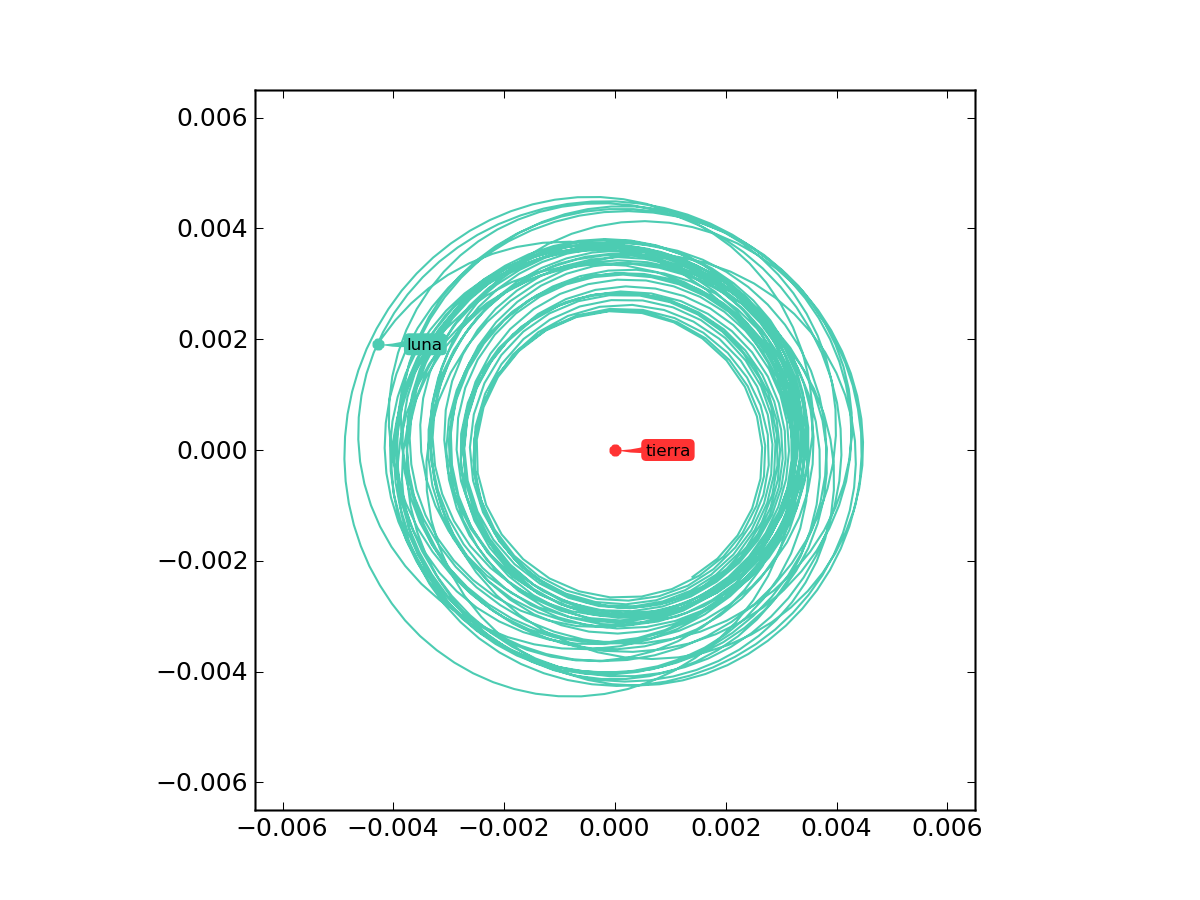
\includegraphics[scale=0.50]{img/zoom_validacion_m1_1000.png}
		\label{fig:rel1}
	}
	\subfigure[metodo = 3, $\Delta t$ = 1 minuto]{
		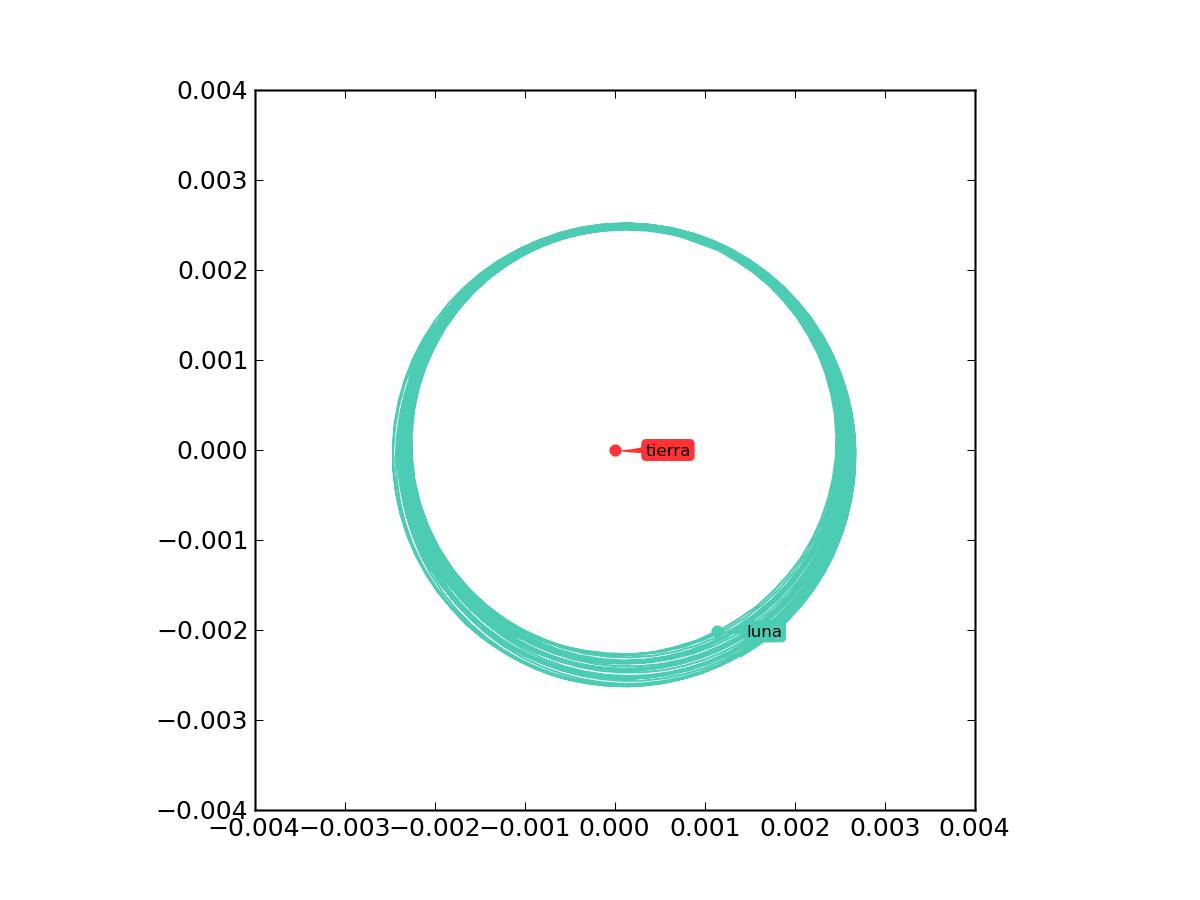
\includegraphics[scale=0.50]{img/validacion_m3_zoom.png}
		\label{fig:rel2}
	}
	\caption{
		Acá vemos 2 ejemplos de la validación del modelo observando en detalle como se comporta la luna relativa a la tierra.
		Simulamos el sistema Sol,Tierra,Luna y graficamos las posiciones de los cuerpos relativos a la posicion de la tierra.
		Vemos que con un $\Delta t$ suficientemente chico la luna gira alrededor de la tierra como esperado.
	}
	\label{ fig:res_ej1_err }
\end{figure}
